\documentclass[border=6pt]{standalone}
\usepackage[T1]{fontenc}
\usepackage[utf8]{inputenc}
\usepackage[scaled=0.98]{helvet}
\renewcommand{\familydefault}{\sfdefault}
\usepackage{amsmath}
\usepackage{graphicx}
\graphicspath{{../../../../../../exercises_lecturenotes/lecture_notes/kurs100_lektionsnoter/}}
\usepackage{tikz}
\usepackage{pgfplots}
\pgfplotsset{compat=1.18}
\usetikzlibrary{arrows.meta, decorations.pathreplacing, calc, positioning, fit, backgrounds, shapes.geometric}
\usepgfplotslibrary{groupplots,fillbetween}
\definecolor{scanpink}{HTML}{E5006D}
\definecolor{scanteal}{HTML}{00A6A6}
\definecolor{scannavy}{HTML}{243746}
\definecolor{scanlightgray}{HTML}{F1F2F3}
\begin{document}
  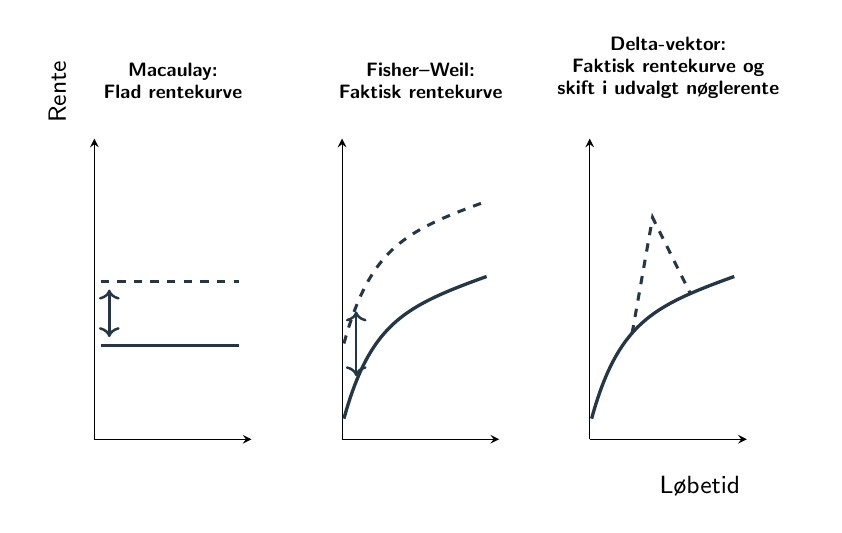
\begin{tikzpicture}
    \begin{groupplot}[
      group style={
        group size=3 by 1,
        horizontal sep=1.15cm
      },
      width=0.295\textwidth,
      height=5.4cm,
      axis lines=left,
      xmin=0,
      xmax=10,
      ymin=0,
      ymax=4.0,
      xtick=\empty,
      ytick=\empty,
      tick label style={font=\scriptsize},
      title style={
        font=\scriptsize\bfseries,
        align=center,
        text width=0.285\textwidth,
        yshift=5pt
      },
      clip=false
    ]

    % -------------------------------------------------
    % Panel 1: Macaulay-varighed
    % -------------------------------------------------
    \nextgroupplot[
      title={Macaulay:\\Flad rentekurve},
      ylabel={Rente},
      ylabel style={
        font=\small,
        rotate=0,
        at={(axis description cs:-0.12,1.02)},
        anchor=south west
      }
    ]

      % Oprindelig flad rentekurve
      \addplot[
        scannavy,
        very thick
      ]
        coordinates {
          (0.4,1.25)
          (9.2,1.25)
        };

      % Parallelt skift
      \addplot[
        scannavy,
        dashed,
        line width=1.1pt
      ]
        coordinates {
          (0.4,2.10)
          (9.2,2.10)
        };

      % Størrelsen på det parallelle rentestød
      \draw[
        <->,
        scannavy,
        line width=0.9pt
      ]
        (axis cs:0.95,1.36)
        --
        (axis cs:0.95,1.99);

    % -------------------------------------------------
    % Panel 2: Fisher--Weil-varighed
    % -------------------------------------------------
    \nextgroupplot[
      title={Fisher--Weil:\\Faktisk rentekurve}
    ]

      % Faktisk nulkuponkurve
      \addplot[
        scannavy,
        very thick,
        domain=0.12:9.2,
        samples=120
      ]
        {0.18 + 1.35*(1-exp(-0.55*x)) + 0.07*x};

      % Parallelt skift af hele nulkuponkurven
      \addplot[
        scannavy,
        dashed,
        line width=1.1pt,
        domain=0.12:9.2,
        samples=120
      ]
        {0.18 + 1.35*(1-exp(-0.55*x)) + 0.07*x + 1.00};

      % Størrelsen på det parallelle rentestød
      \draw[
        <->,
        scannavy,
        line width=0.9pt
      ]
        (axis cs:0.90,0.84)
        --
        (axis cs:0.90,1.70);

    % -------------------------------------------------
    % Panel 3: Delta-vektor
    % -------------------------------------------------
    \nextgroupplot[
      title={Delta-vektor:\\Faktisk rentekurve og\\skift i udvalgt nøglerente},
      xlabel={Løbetid},
      xlabel style={
        font=\small,
        at={(axis description cs:1.02,-0.09)},
        anchor=north east
      }
    ]

      % Faktisk nulkuponkurve
      \addplot[
        scannavy,
        very thick,
        domain=0.12:9.2,
        samples=120
      ]
        {0.18 + 1.35*(1-exp(-0.55*x)) + 0.07*x};

      % Lokalt trekantet stød til én nøglerente
      \addplot[
        scannavy,
        dashed,
        line width=1.1pt
      ]
        coordinates {
          (2.70,1.41)
          (4.00,2.95)
          (6.40,1.94)
        };

    \end{groupplot}
  \end{tikzpicture}
\end{document}
